\section{Teoría del flujo unidimensional}


\subsection{Sistema y volumen de control}

\subsubsection{Sistema de control}
Un sistema de control se refiere a una masa fija (infinitesimal o finita) definida y se distingue de todas las demás. Las fronteras del sistema forman una superficie cerrada. Esta superficie puede variar en el tiempo de tal manera que mantenga la misma masa durante los cambios. Es decir $dm/dt = 0$.
En el enfoque \emph{Lagrangiano} en el cual el estudio se centra en el movimiento de partículas individuales, el movimiento se observa como una función del tiempo. Es decir se "sigue" a la partícula, como en el estudio de sólidos. En este caso se utiliza un sistema de control, ya que la masa de la partícula o solido se mantiene constante

\begin{figure}[h]
	\centering
	\begin{subfigure}[b]{.45\linewidth}
		\centering
		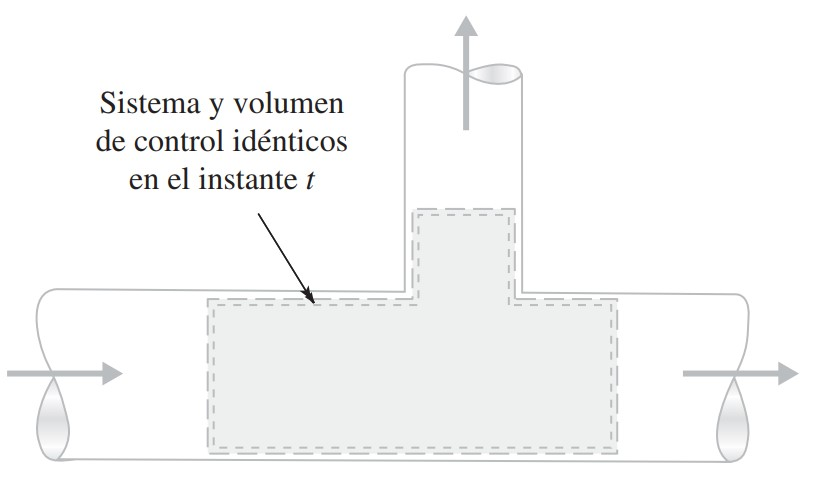
\includegraphics[width = .6\linewidth]{U3-sistema-volumen-control}
		\label{fig:manometro-u}
	\end{subfigure}
	\begin{subfigure}[b]{.45\linewidth}
		\centering
		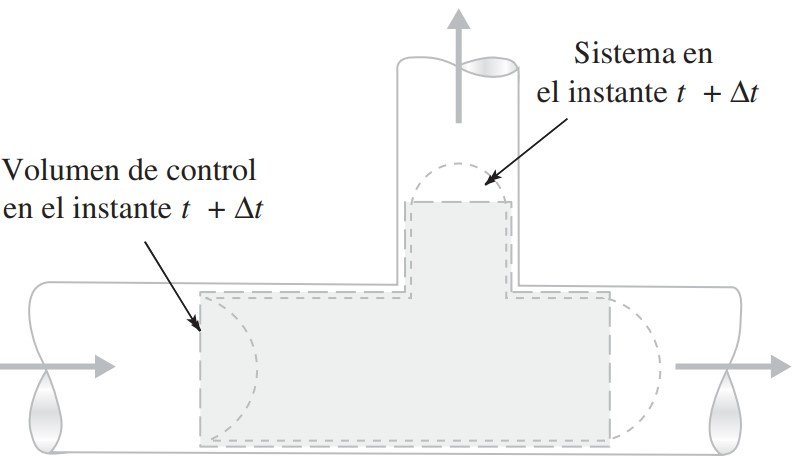
\includegraphics[width = .6\linewidth]{U3-sistema-volumen-control2}
		\label{fig:manometro-u2}
	\end{subfigure}
	\caption{Sistema y volumen de control}
\end{figure}

\subsubsection{Volumen de control}
En el enfoque \emph{Euleriano} se mantiene fija la coordenada espacial y así se pueden observar las velocidades de las partículas móviles al pasar por esta posición en cualquier instante. Entonces, las propiedades del flujo son funciones del espacio y el tiempo.
Este tipo de enfoque se puede estudiar a través de un volumen de control o punto fijo, en el cual el flujo pasa a traces de este.

%%%%%%%%%%%%%%%%%%%%%%%%%%%%%%%%%%%%%%%%%%%%%%%%%%%%%%
\subsection{Linea y tubo de corriente}

\subsubsection{Linea de trayectoria}
Es el lugar geométrico de los puntos recorridos por una partícula determinada cuando se desplaza en un campo de flujo.

\subsubsection{Linea de corriente}
Es una línea continua que representa el flujo y ésta posee la propiedad de que el vector velocidad de cada partícula es tangente a la línea de corriente. La ecuacion que representa el vector: $ \overline{v} \times d\overline{r} = 0$

\begin{figure}[h]
	\centering
	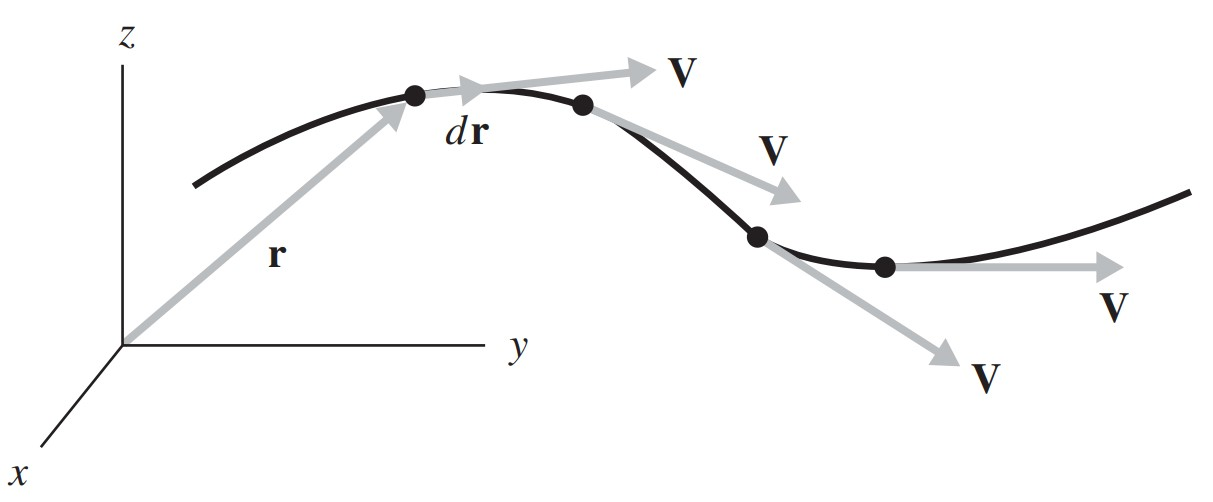
\includegraphics[width = .5\linewidth]{U3-linea-corriente}
	\caption{Linea de corriente en un campo de flujo}
\end{figure}

En un flujo \emph{permanente} la trayectoria de una partícula es una linea de corriente. Pero en un flujo no permanente donde el vector velocidad cambia con el tiempo, haciendo que la partícula siga diferentes lineas de corrientes de tal manera que la trayectoria de esta no puede parecerse a ninguna linea de corriente.

\subsubsection{Tubo de corriente}
Un tubo de corriente está constituido por una región parcial del flujo delimitada por una familia de lineas de corriente. No existe flujo a través de las paredes ya que el vector velocidad no tiene componete perpendicular a la superficie del tubo ya que siempre es tangente a la linea de corriente.

%%%%%%%%%%%%%%%%%%%%%%%%%%%%%%%%%%%%%%%%%%%%%%%%%%%%%%%%%%%%%%%
\subsection{Tipos de flujo}
\subsubsection{Flujo permanente}
Ocurre cuando las condiciones en cualquier punto del fluido no cambian con el tiempo es decir:

\begin{tabular}{r c l}
	\centering
	$\dfrac{\delta v}{\delta t} = 0$ & $\dfrac{\delta p}{\delta t} =0$ & $ \dfrac{\delta \rho}{\delta t}=0$
\end{tabular}

Esto no significa que la velocidad no varíe de un punto.

\subsubsection{Flujo en una, dos y tres dimensiones}
El vector velocidad del flujo $\vec{V}$ puede depender de una, dos o tres dimensiones espaciales mas el tiempo. El nombre que recibe el flujo dependiendo de cuantas variables espaciales depende es: \textbf{unidimesional}(tubos largos, rectos, o entre placas), \textbf{bidimensional} o \textbf{tridimensional}. 


El flujo en una dimensión no tiene en cuenta las variaciones o cambios en la velocidad, presión, etc. en un plano transversal a la dirección de este, es decir, el vector velocidad depende solo de una variable espacial.



\subsubsection{Flujo laminar y turbulento}

En un \textbf{flujo laminar} las partículas se mueven a lo largo de trayectorias suaves en láminas o capas, con una capa deslizándose suavemente sobre otra adyacente. El flujo laminar está gobernado por la ley de viscosidad de Newton, la cual relaciona el esfuerzo cortante con la tasa de deformación angular. En situaciones de baja viscosidad, alta velocidad o grandes caudales, este flujo no es estable y se rompe en flujo turbulento.\\

En un \textbf{flujo turbulento} los movimientos del fluido varían irregularmente. Las partículas se mueven en trayectorias arremolinadas causando un intercambio de momentum. La turbulencia causa mayores esfuerzos cortantes y pérdidas.\\

Si un flujo es laminar o turbulento depende de tres parámetros físicos que combinados forman el número de \textbf{Reynolds} y nos permite determinar el régimen de flujo:\\

\begin{tabular}{c c}
		\begin{minipage}[t]{.45\textwidth}
			\flushright 
			\vspace{.05cm}
			$Re= \dfrac{V L}{\nu}$
		\end{minipage}
		&
		\begin{minipage}[t]{.45\textwidth}
			\flushleft
			V velocidad\\
			L Longitud\\
			$\nu$ viscosidad cinemática
		\end{minipage}
\end{tabular}

\subsubsection{Flujos viscosos e inviscidos}
El \textbf{flujo inviscido} es aquel en donde se desprecian los efectos viscosos. Estos flujos se consideran generalmente en flujos externos, para el estudio de flujos aerodinámicos, donde los efectos viscosos están confinados en una capa delgada alrededor del cuerpo denominada \emph{capa límite}. \\

En un \textbf{flujo viscoso} se consideran las pérdidas que generan los efectos viscosos. Esto suele ocurrir en tubos, conductos, o canales abiertos. 

\subsubsection{Flujo compresible e incompresible}
		
Un \textbf{flujo incompresible} existe si la densidad de cada partícula de fluido permanece relativamente constante cuando se mueve por el campo del fluido.
\begin{equation*}
	\dfrac{D \rho}{dt} = 0
\end{equation*}

Esta condición no implica que la densidad sea la misma en todos los puntos.

En flujos de gas, el número de Mach nos permite determinar si este flujo puede ser estudiado como compresible ($M < 0.3$) o incompresible.

\begin{equation*}
	M = \dfrac{V}{c}
\end{equation*}

donde $V$ es la velocidad del gas y $c=\sqrt{k R T}$ es la velocidad de la onda.\\


En un \textbf{flujo compresible}.. avisale


\subsection{Ecuación de continuidad}

La \textbf{ley de conservación de la masa} establece que toda la masa de un sistema permanece constante, en otras palabras, el caudal de flujo permanece constante a lo largo del trayecto.\\


Considerando un caudal volumétrico de un flujo con densidad constante entre dos puntos (1) y (2):
\begin{equation*}
	Q_1 = Q_2 \left[\dfrac{m^3}{s}\right]
\end{equation*}

además, si se considera el caudal en función de la sección transversal del flujo y la velocidad de las partículas en ese punto, se llega a la \emph{ecuación de la continuidad}:

\begin{equation}
	A_1  V_1 = A_2 V_2
	\label{eq:continuidad-1}
\end{equation}


En caso de que se presenten perfiles de velocidad no uniformes, como se muestra en la figura \ref{fig:velocidad-no-uniforme}, se toma la velocidad promedio en el instante determinado y se denota con una raya arriba. La ecuación de continuidad se expresa entonces

\begin{equation}
	A_1 \overline{V}_1= A_2  \overline{V}_2
	\label{eq:continuidad-2}
\end{equation} 

\begin{figure}[H]
	\centering
	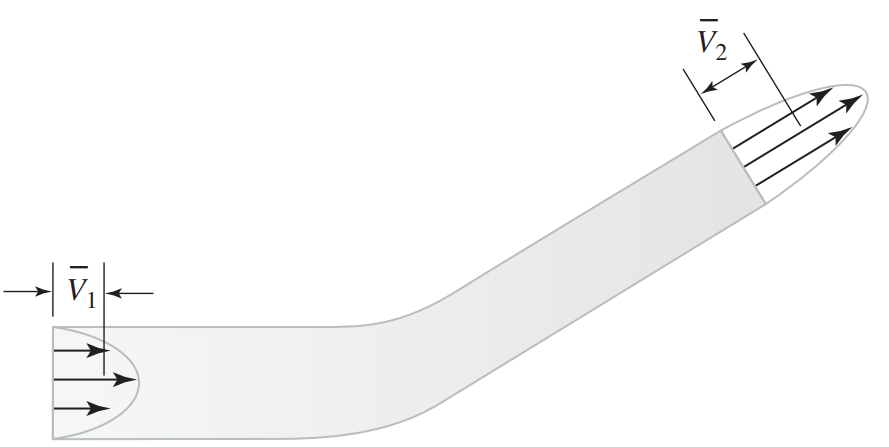
\includegraphics[width=.5\linewidth]{U3-velocidad-no-uniforme}
	\caption{Perfiles de velocidad no uniformes.}
	\label{fig:velocidad-no-uniforme}
\end{figure}


\subsection{Ecuación de Bernoulli}
\subsubsection{Enfoque diferencial}

Para la deducción de la \emph{ecuación de Bernoulli} se realizaron cinco suposiciones:
\begin{itemize}
	\item Flujo inviscido (sin esfuerzos cortantes)\vspace{-.2cm}
	\item Flujo permanente ($\partial V / \partial t = 0$)\vspace{-.2cm}
	\item A lo largo de una línea de corriente ($a_s = V \partial V / \partial s$)\vspace{-.2cm}
	\item Densidad constante ($\partial \rho / \partial s = 0$)\vspace{-.2cm}
	\item Marco de referencia inercial.
\end{itemize}

Teniendo en cuenta la ecuación de \textbf{Euler} a lo largo de una linea de corriente:
\begin{equation}
	\dfrac{dp}{\rho} + g dz + v dv = 0
\end{equation}

Ecuación que se obtiene a partir de considerar un volumen de control diferencial que es atravesado por una linea de corriente. (Streeter U4)
Se puede integrar esta ecuación y nos quedaría:

\begin{equation}
	g z + \dfrac{v^{2}}{2} + \dfrac{p}{\rho} = constante
\end{equation}

Donde la constante se conoce como \emph{constante de Bernoulli}. \\

La ecuación se conoce también como ecuacion de la conservación de energía mecánica.
\subsubsection{Enfoque termodinámico}

Para el siguiente análisis se plantea la \emph{primera ley de la termodinámica} para un sistema de régimen permanente esquematizado en la figura \ref{fig:ecuacion-de-bernoulli}, donde la ecuación de flujo estable se puede expresar como sigue:

\begin{equation*}
 \dfrac{p_1}{\rho} +	\dfrac{V_1^2}{2} + g z_1 + u_1 + Q=  \dfrac{p_2}{\rho} + \dfrac{V_2^2}{2} + g z_2 + u_2 + W
\end{equation*}


Si las pérdidas son insignificantes y no se suministra ni se extrae energía del sistema, tanto la energía interna $u$, como el calor $Q$ y trabajo $W$ se eliminan de la ecuación, obteniendo entonces la \emph{ecuación de Bernoulli}:

\begin{equation}
	\dfrac{p_1}{\rho} +	\dfrac{V_1^2}{2} + g z_1 =  \dfrac{p_2}{\rho} + \dfrac{V_2^2}{2} + g z_2
	\label{eq:bernoulli}
\end{equation}

\begin{figure}[H]
	\centering
	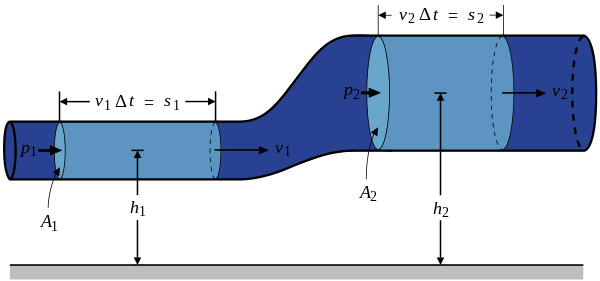
\includegraphics[width = .5 \linewidth]{U3-flujo-bernoulli}
	\caption{Esquema del principio de Bernoulli}
	\label{fig:ecuacion-de-bernoulli}
\end{figure}

Vemos entonces como llegamos a la misma ecuación desde dos puntos diferentes de vista.

\subsubsection{Efecto Venturi}

\subsection{Cantidad de movimiento}

La segunda Ley de Newton establece

\begin{equation*}
	\vec{F} = \dfrac{d(m \vec{v})}{dt} = \dfrac{d}{dt} \int_{vc} \rho (\vec{v} \cdot \widehat{n}) dV + \int_{sc} \vec{v} \rho \vec{v} dA
\end{equation*}

En el cual la suma vectorial de fuerzas externas que actúan sobre el volumen de control es igual a la razón de cambio de la cantidad de movimiento dentro del volumen de control mas la razón de cambio neto a la cual la cantidad de movimiento está dejando la superficie de control. El vector $\widehat{n}$ es el vector de área y siempre apunta hacia afuera de ésta.\\

Para un flujo permanente uniforme, la primer integral se hace cero entonces:

\begin{equation}
	\sum \vec{F} = \sum_{i = 1}^{N} \rho_{i} A_{i} \vec{v_{i}} (\vec{v_{i}} \cdot \widehat{n})
\end{equation}

Donde N es el número de áreas de entrada o salida de flujo. Si tenemos en cuenta que el flujo másico es $\dot{m} = \rho A v$ se puede simplificar la ecuación.


%%%%%%%%%%%%%%%%%%%%%%%%%%%%%%%%%%%%%%%%%%%%%%%%%%%%%%%%%%%%
